\label{sec:discussion:subsec:convergence}

\section{Discussion}
\label{sec:evaluation}

\begin{comment}
\todo[inline]{CDC: MISSING:
Nella evaluation, dobbiamo riportare l'uso di memoria qui conta perché è un parametro fondamentale.
\\
Dobbiamo informare il lettore sulle caratteristiche del log (numero eventi, numero tracce, dimensione totale in KB una volta salvato in formato XES), come lo abbiamo creato, perché il modello non è uguale a quello di Fig. 1.}
\end{comment}


In this section, we evaluate the proposed approach. In the first paragraph of the section  we delve into a convergence analysis by evaluating the correctness of the collaborative data exchange process. Subsequently, we took into assessment the memory usage by measuring the RAM usage associated with the execution of the \Compo{Secure Miner} components, using diverse parameter configurations.
\begin{figure}[t]
	\subfloat[][Workflow net mined from the Pharmaceutical company log.]{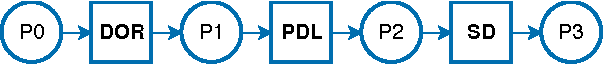
\includegraphics[width=0.37\linewidth]{content/figures/pharma_dep1.pdf}\label{fig:wfnet:a}}
	\hfill
	\subfloat[][Workflow net mined from the Specialized clinic log.]{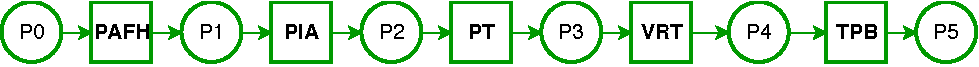
\includegraphics[width=0.57\linewidth]{content/figures/specialised_dep1.pdf}\label{fig:wfnet:b}}
	\hfill
	\vspace{1em}
	\subfloat[][Workflow net mined from the Hospital log.]{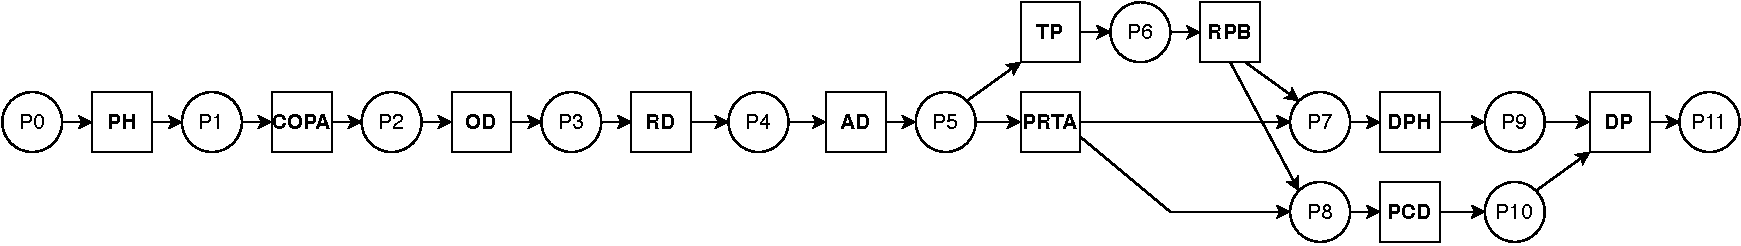
\includegraphics[width=1\linewidth]{content/figures/hospital_dep1.pdf}\label{fig:wfnet:c}}
	\hfill
	\vspace{1em}
	\subfloat[][Workflow net mined from the merged log in our inter-organizational setting.]{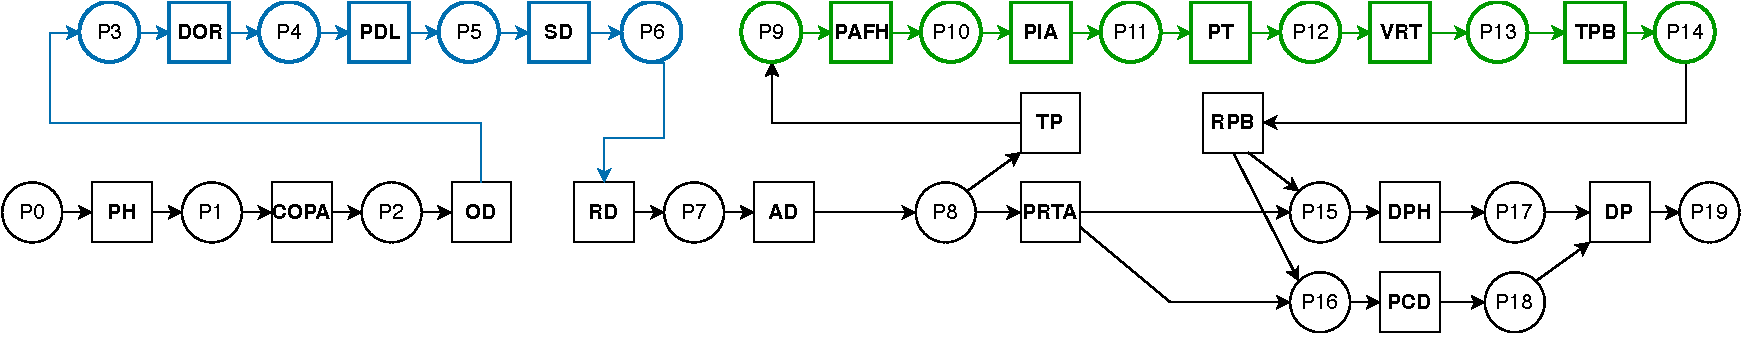
\includegraphics[width=1\linewidth]{content/figures/merged_dep1.pdf}\label{fig:wfnet:d}}
	\caption{Outputs of the HeuristicsMiner used for the convergence test.}
	\label{fig:wfnet}
\end{figure}

\textbf{Convergence of the outputs.}
\label{sec:discussion:subsec:convergence}
We assess the convergence of the \textit{HeuristicsMiner} outcomes as a means of validating the correct functioning of the event log transmission mechanism. Specifically, we generated workflow net outputs by applying intra-organizational mining procedures, wherein each organization independently mined its event log. Subsequently, we employed our approach with a miner actor conducting the \textit{HeuristicsMiner} algorithm using an inter-organizational event log obtained as a result of the log exchange and merging mechanisms. Finally, we compared the results obtained through our approach with the single outputs mined using the partial event log in intra-organizational setting.  For the purpose of this test, we utilize the synthetic event log based on our motivating scenario, which features a corresponding BPMN diagram (as depicted in \cref{fig:BPMN_Healthcare}). Upon careful examination of \cref{fig:wfnet}, we show that the workflow net generated by the \textit{HeuristicsMiner} in our approach, as displayed in \cref{fig:wfnet:d}, encapsulates the structure and behavior observed in the workflow nets produced by the intra-organizational \textit{HeuristicsMiner} execution. In specific terms, the blue-colored part in \cref{fig:wfnet:d} reflects the behavior of the \Actor{Pharmaceutical company}, depicted in \cref{fig:wfnet:a}, commencing from the moment the drug order is received to its fulfillment. Furthermore, the green-colored part delineates the process of the \Actor{Specialized clinic}, starting from the patient's arrival from the \texttt{Hospital} to their transfer described in \cref{fig:wfnet:b}. Finally, the black-colored portion of the workflow net is consistent with the output resulting from the partial log of the \Actor{Hospital} showed in \cref{fig:wfnet:c}.

\begin{table}[t!]%\hskip-2.5cm
  \caption{Tested event logs.}
 \centering
    \begin{minipage}[t]{1\linewidth}
    %\subfloat{% Subtable 1
       \resizebox{0.98\textwidth}{!}{%
            \begin{tabular}{l|l|l|l|l}
            \textbf{Name}                & \textbf{Synthetic/Real} & \textbf{Max events} & \textbf{Cases} & \textbf{Organizations} \\ \hline
            Motivating Scenario (MS\_0) & Synthetic      & 19         & 1000   & 3             \\
            Sepsis & Real      & 19         & 4000   & 1             \\
            BPIC2013 & Real      & 35         & 1432    & 3             \\
            \end{tabular}
        }% resizebox
    %}% subfloat
    \end{minipage}%
\end{table}
\begin{figure}[t!]
    \subfloat[][Memory usage at runtime.]{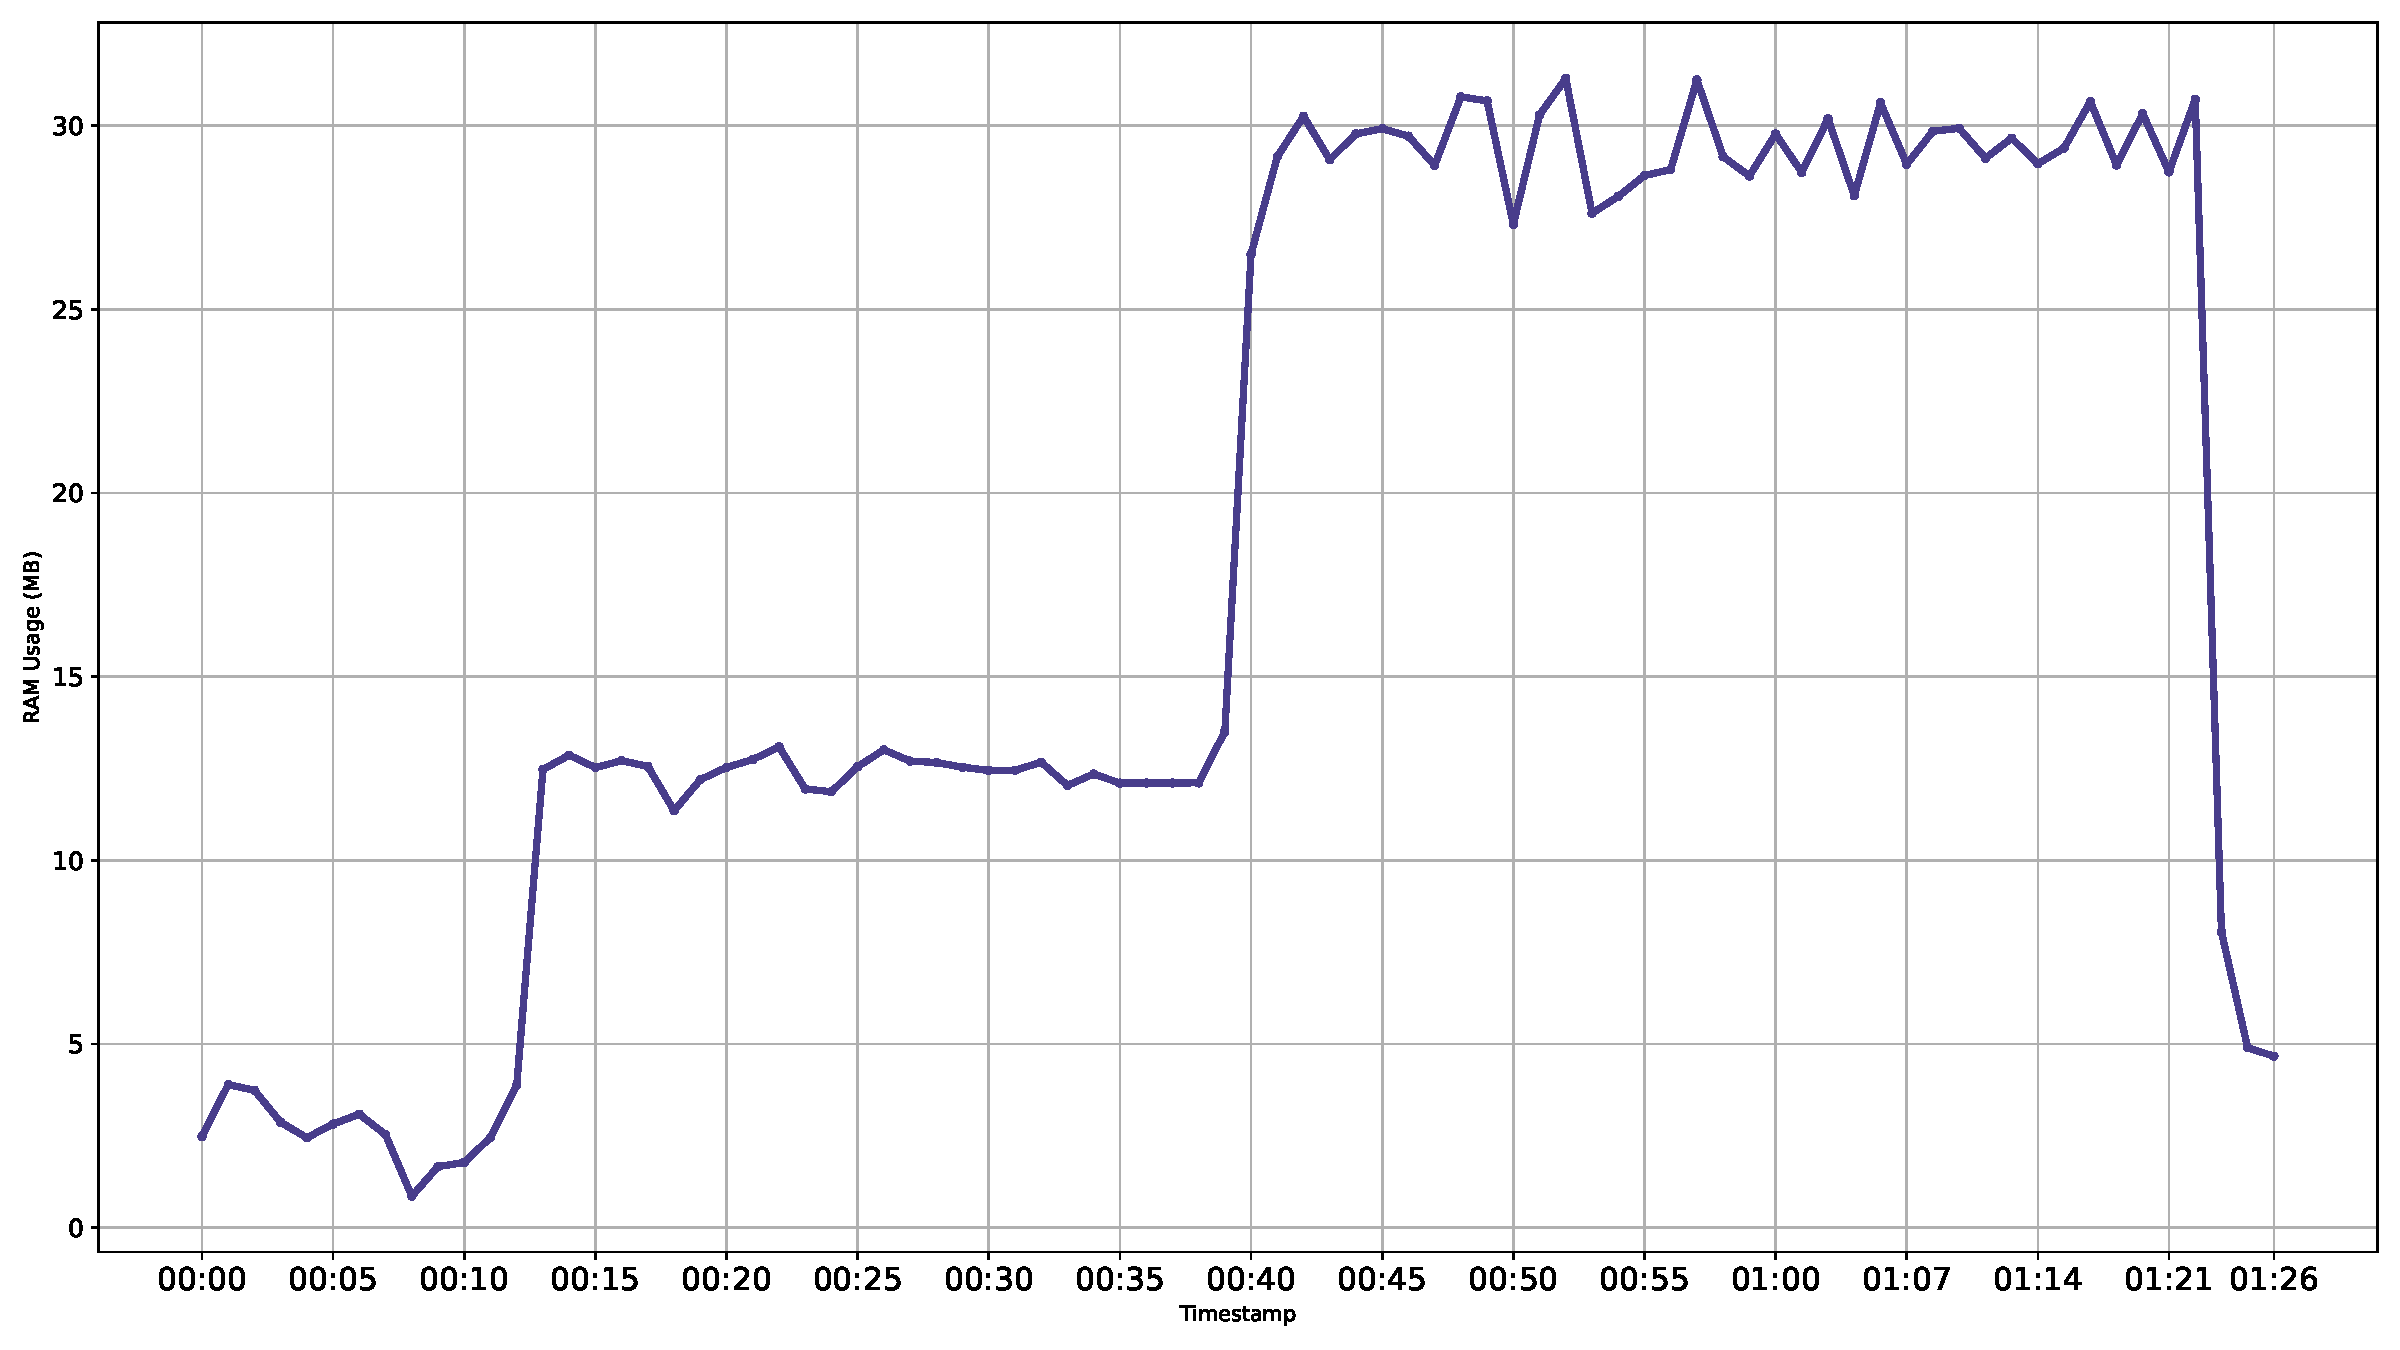
\includegraphics[width=0.48\linewidth]{content/figures/ram_usage_per_TS.pdf}\label{fig:wfnet:a}}
        \hfill
    \subfloat[][Memory usage as segment size increases.]{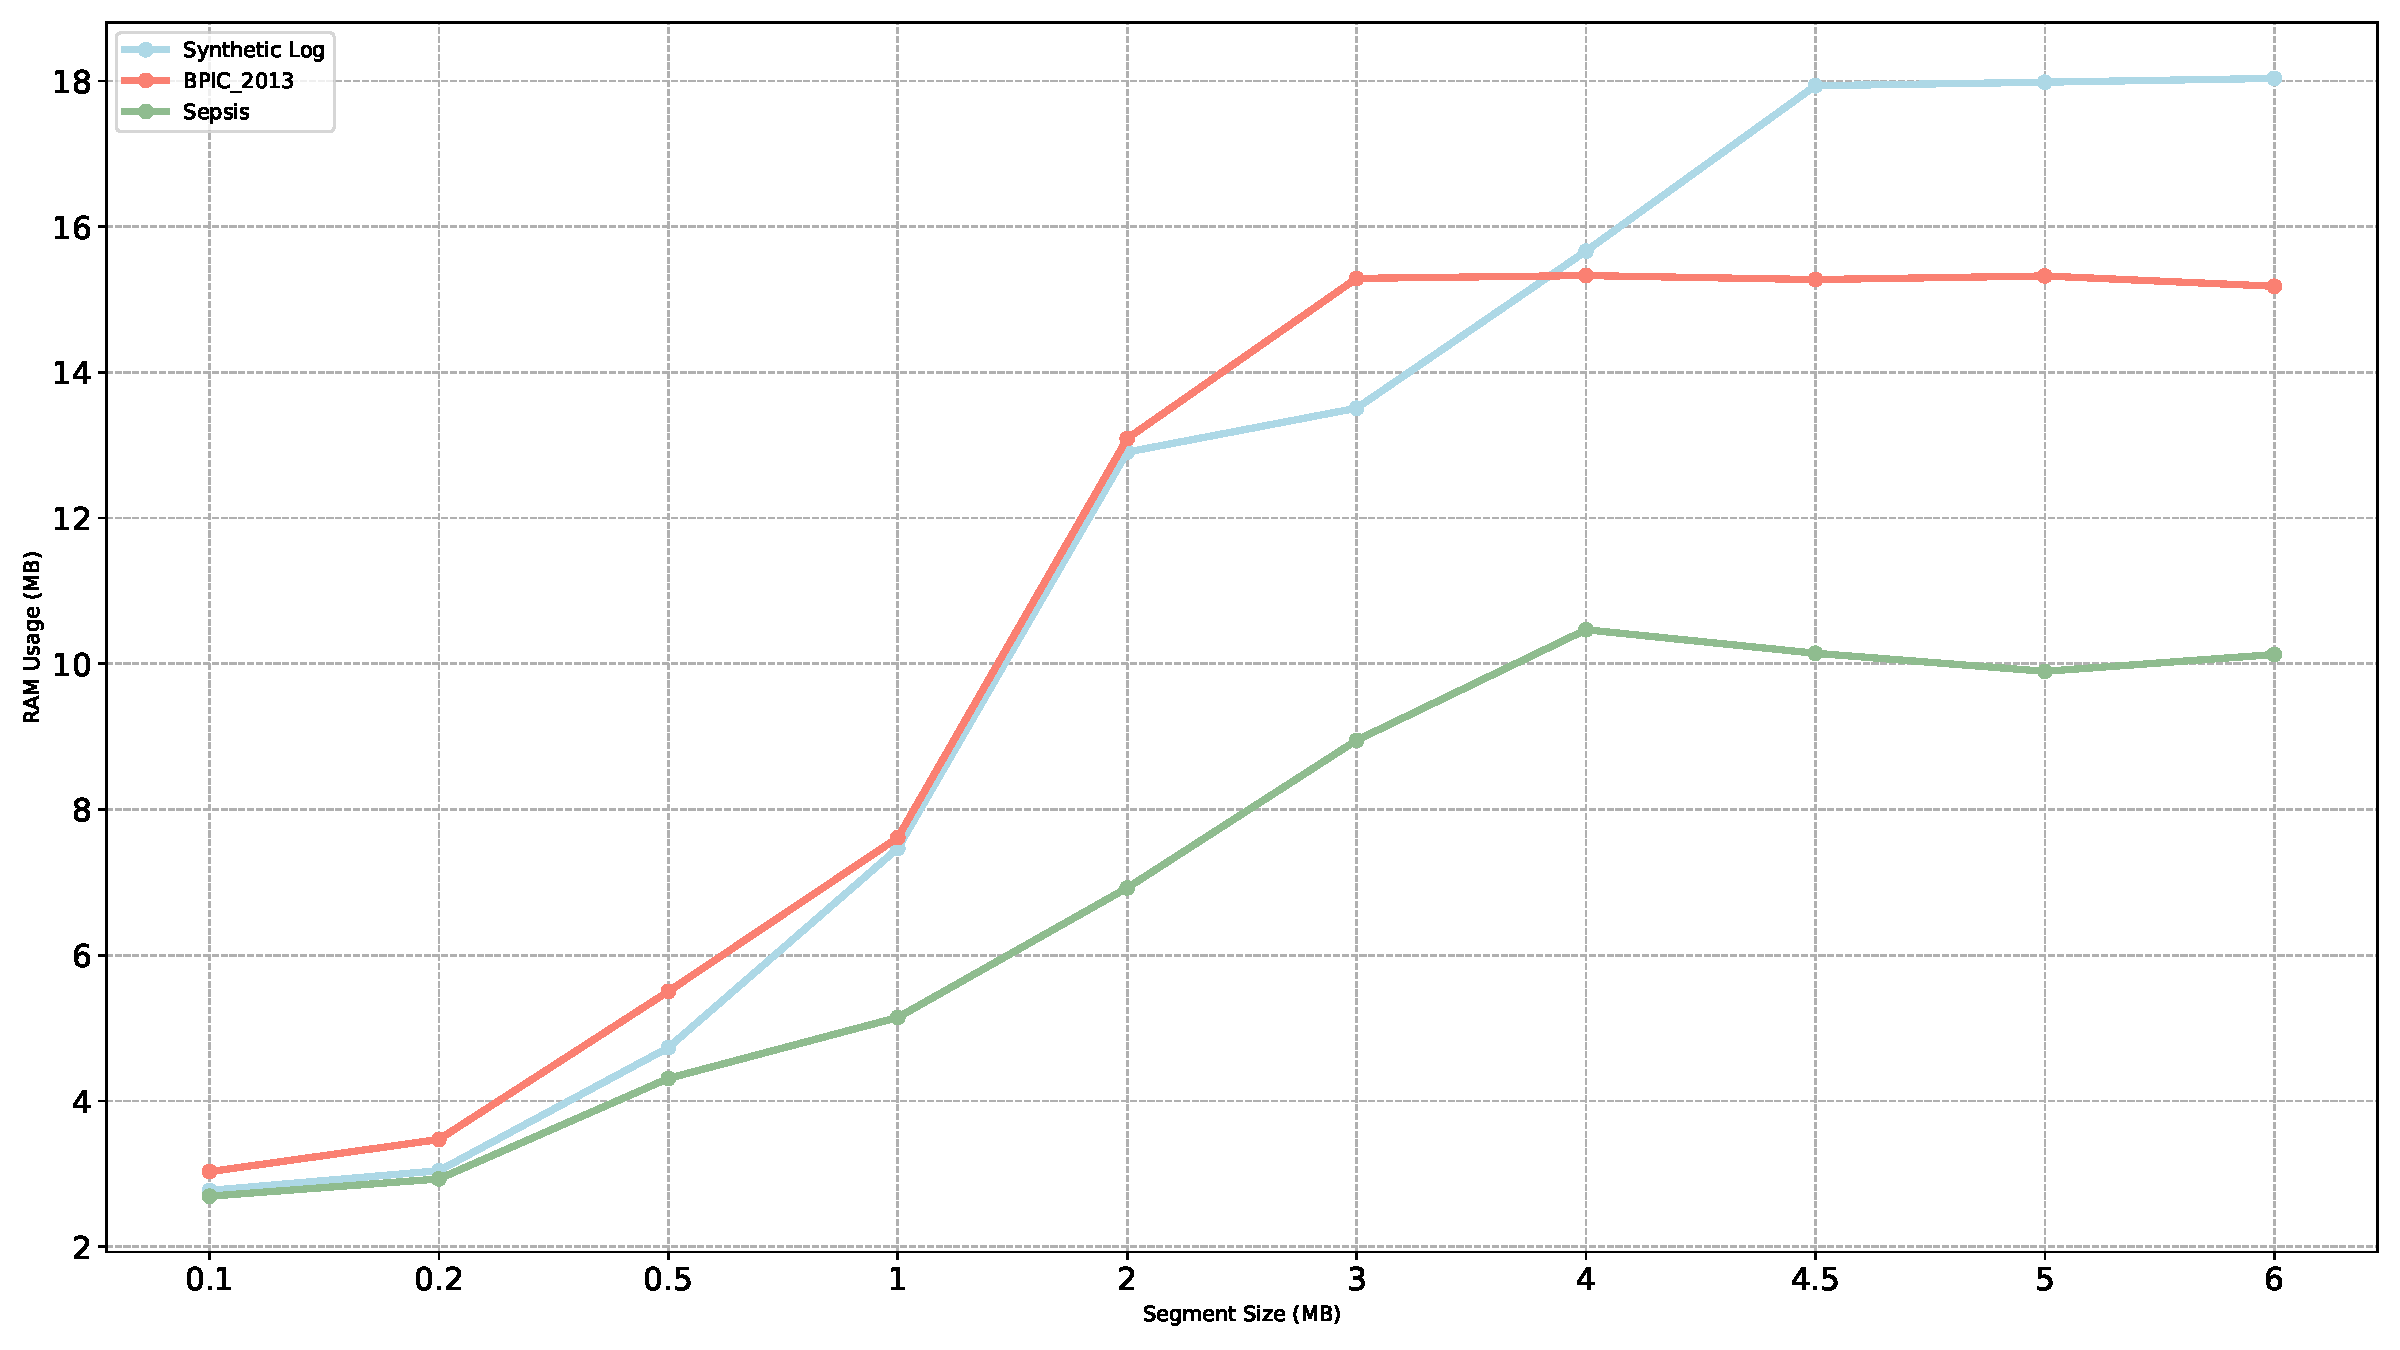
\includegraphics[width=0.48\linewidth]{content/figures/lineplot_segsize_combined.pdf}\label{fig:wfnet:b}}
    \caption{Memory usage tests.}
    \label{fig:wfnet}
\end{figure}
\begin{figure}[t!]
    \subfloat[][FIGURE TO BE REPLACED WITH LINEPLOT (THROUGHPUT;n°organizaitons)]{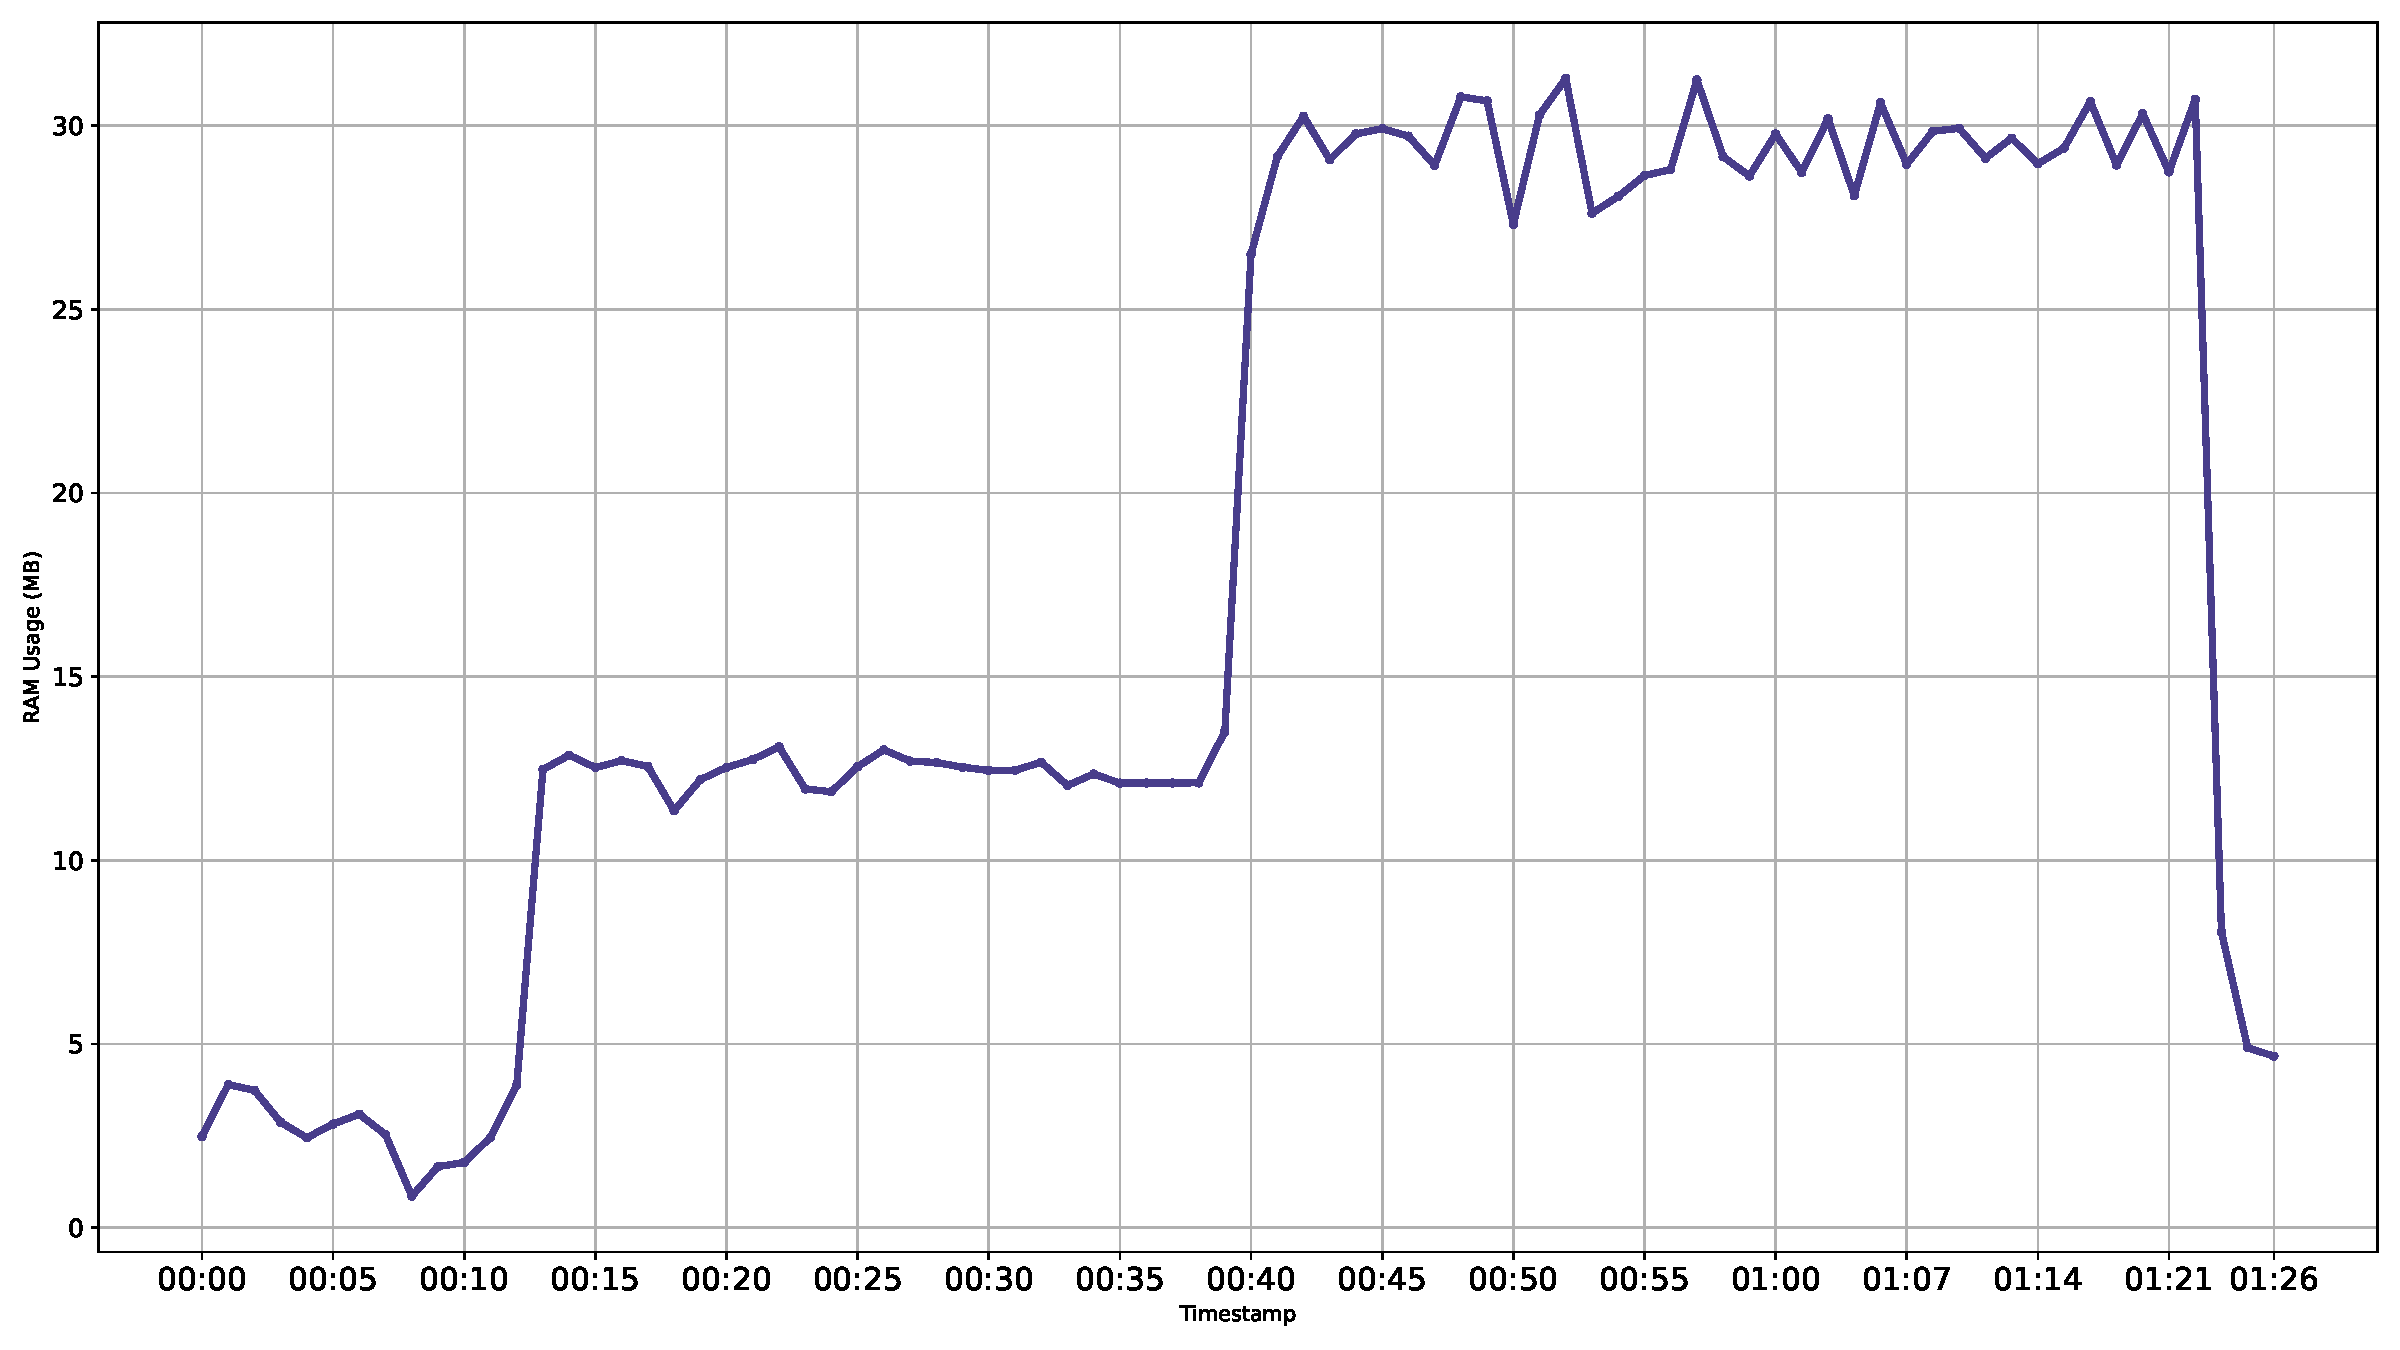
\includegraphics[width=0.48\linewidth]{content/figures/ram_usage_per_TS.pdf}\label{fig:wfnet:a}}
        \hfill
    \subfloat[][FIGURE TO BE REPLACED WITH LINEPLOT(RAM;n°organizations)]{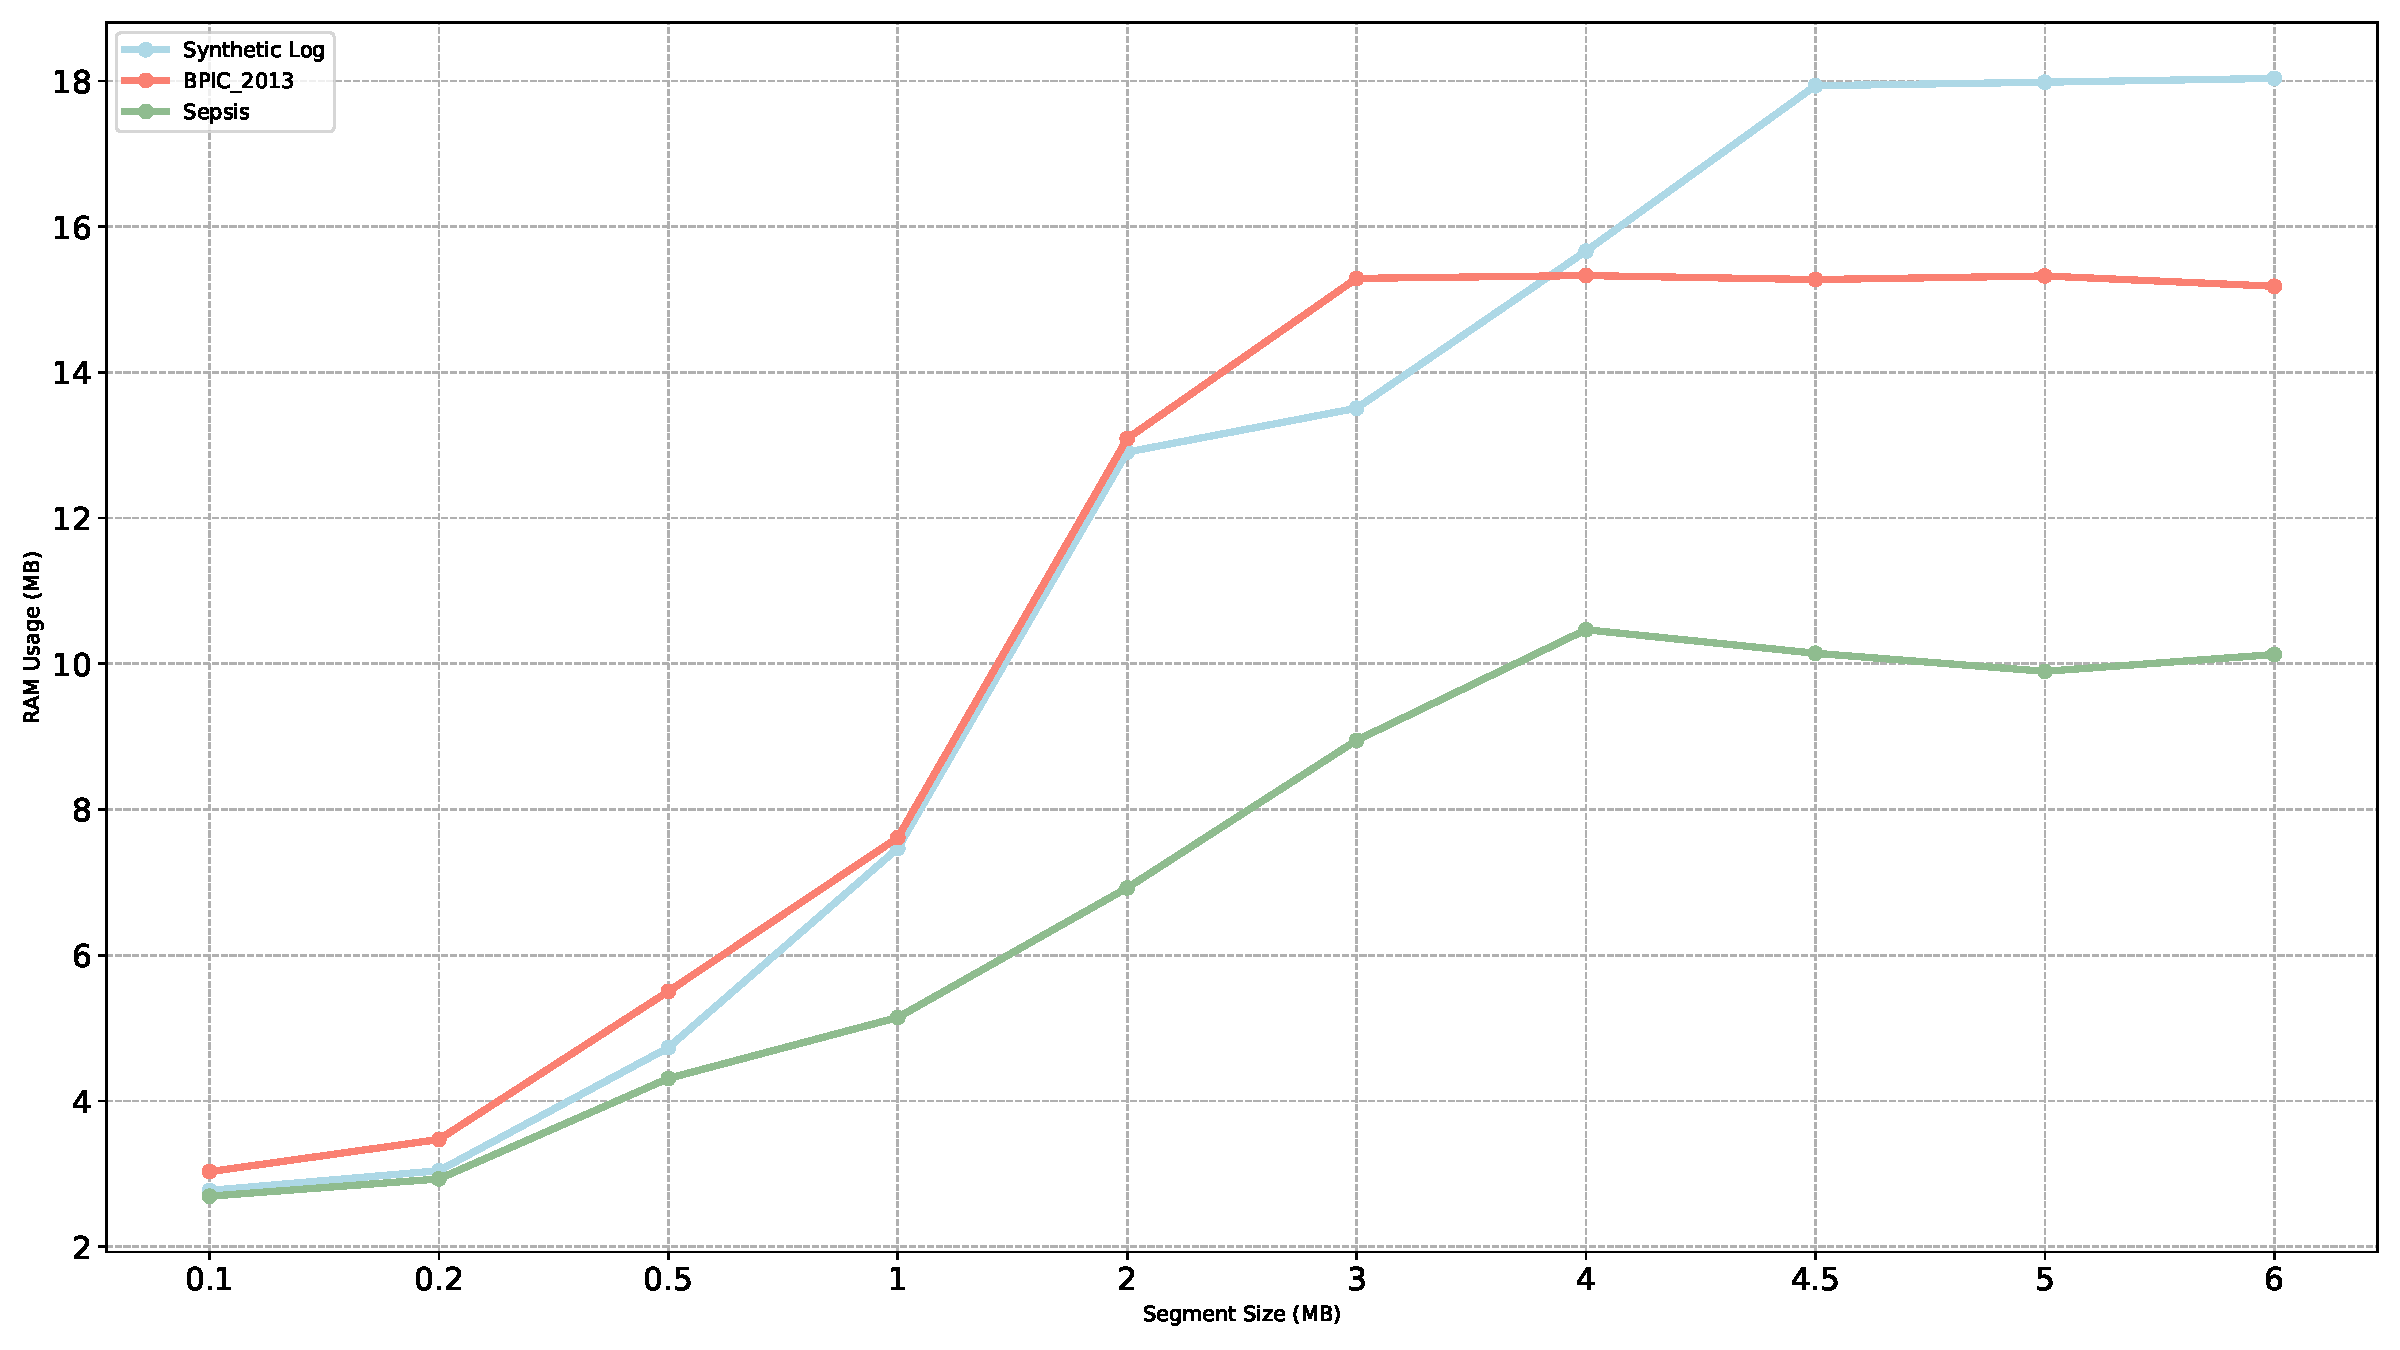
\includegraphics[width=0.48\linewidth]{content/figures/lineplot_segsize_combined.pdf}\label{fig:wfnet:b}}
    \caption{FIGURE FOR SCALABILITY TEST TO BE REPLACED}
    \label{fig:wfnet}
\end{figure}

\textbf{Memory Usage.}

\textbf{Scalability.}